\documentclass{article}
\usepackage{amsmath,amsfonts,amsthm,amssymb,amsopn,bm}
\usepackage[margin=.9in]{geometry}
\usepackage{graphicx}
\usepackage{url}
\usepackage[usenames,dvipsnames]{color}
\usepackage{fancyhdr}
\usepackage{multirow}
\usepackage{listings}
\usepackage{hyperref}

\definecolor{keywords}{RGB}{255,0,90}
\definecolor{comments}{RGB}{0,0,113}
\definecolor{red}{RGB}{160,0,0}
\definecolor{green}{RGB}{0,150,0}
 
\lstset{language=Python, 
        basicstyle=\ttfamily\tiny, 
        keywordstyle=\color{keywords},
        commentstyle=\color{comments},
        stringstyle=\color{red},
        showstringspaces=false}

\newcommand{\argmax}{\arg\!\max}
\newcommand{\argmin}{\arg\!\min}
\newcommand{\field}[1]{\mathbb{#1}}
\newcommand{\1}{\mathbf{1}}
\newcommand{\E}{\mathbb{E}} 
\renewcommand{\P}{\mathbb{P}}
\newcommand{\R}{\field{R}} % real domain
% \newcommand{\C}{\field{C}} % complex domain
\newcommand{\F}{\field{F}} % functional domain
\newcommand{\T}{^{\textrm T}} % transpose
\def\diag{\text{diag}}

%% operator in linear algebra, functional analysis
\newcommand{\inner}[2]{#1\cdot #2}
\newcommand{\norm}[1]{\left\|#1\right\|}
\newcommand{\twonorm}[1]{\|#1\|_2^2}
% operator in functios, maps such as M: domain1 --> domain 2
\newcommand{\Map}[1]{\mathcal{#1}}
\renewcommand{\theenumi}{\alph{enumi}} 


\newcommand{\Perp}{\perp \! \! \! \perp}

\newcommand\independent{\protect\mathpalette{\protect\independenT}{\perp}}
\def\independenT#1#2{\mathrel{\rlap{$#1#2$}\mkern2mu{#1#2}}}
\newcommand{\vct}[1]{\boldsymbol{#1}} % vector
\newcommand{\mat}[1]{\boldsymbol{#1}} % matrix
\newcommand{\cst}[1]{\mathsf{#1}} % constant
\newcommand{\ProbOpr}[1]{\mathbb{#1}}
\newcommand{\points}[1]{\small\textcolor{magenta}{\emph{[#1 points]}} \normalsize}
\date{{}}

\setlength\parindent{0px}

\begin{document}
\title{Homework \#1 B}
\author{\normalsize{Spring 2020, CSE 446/546: Machine Learning}\\
\normalsize{Dino Bektesevic}}
\maketitle

\section*{Ridge regression on MNIST}
B.2 
\begin{enumerate}
    \item \points{10} We just fit a classifier that was linear in the pixel intensities to the MNIST data. For classification of digits the raw pixel values are very, very bad features: it’s pretty hard to separate digits with linear functions in pixel space. The standard solution to this is to come up with some transform $h:\R^d\rightarrow \R^p$ of the original pixel values such that the transformed points are (more easily)linearly separable. In this problem, you’ll use the feature transform:
    
    $$h(x) = \cos(Gx+b)$$
    
    where $G\in R^{p\times d}$, $b\in \R^p$, and the cosine function is applied element wise. We’ll choose $G$ to be a random matrix, with each entry sampled i.i.d. from a Gaussian with mean $\mu = 0$ and variance $\sigma^2=0.1$, and $b$ to be a random vector sampled i.i.d. from the uniform distribution on $[0, 2\pi]$. The big question is: how do we choose $p$? Using cross-validation, of course! Randomly partition your training set into proportions 80/20 to use as a new training set and validation set, respectively. Using the train function you wrote above, train $\widehat W_p$ for different values of $p$ and plot the classification training error and validation error on a single plot with $p$ on the x-axis. Be careful, your computer may run out of memory and slow to a crawl if $p$ is too large ($p\leq 6000$ should fit into 4 GB of memory that is a minimum for most computers, but if you’re having trouble you can set $p$ in the several hundreds). You can use the same value of $\lambda = 1e-4$ as above but feel free to study the effect of using different values of $\lambda$ and $\sigma^2$ for fun.
    
    \begin{center}
    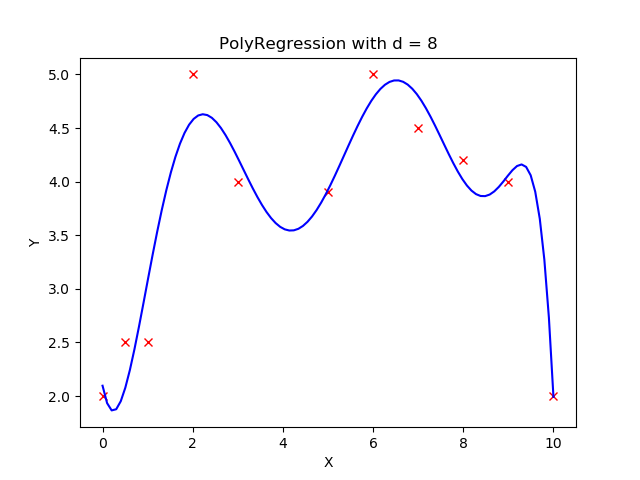
\includegraphics[width=4in]{HW1/HW1_plots/PolyFit.png}
    \end{center}    
    
    \item \points{5} Instead of reporting just the test error, which is an unbiased estimate of the true error, we would like to report a confidence interval around the test error that contains the true error. 
    
    Lemma 1. (Hoeffding’s inequality) Fix $\delta\in (0,1)$. If for all $i=1,\hdots,m$ we have that $X_i$ are i.i.d.random variables with $X_i\in [a,b]$ and $\E[X_i]=\mu$ then
    
    $$P\left(\left| \left(\frac{1}{m}\sum_{i=1}^m X_i\right) - \mu\right| \geq \sqrt{\frac{(b-a)^2 \log(2/\delta)}{2m}} \right) \leq \delta$$
    
    We will use the above equation to construct a confidence interval around the true classification error ($\hat f=\E_\text{test}[\widehat\epsilon_\text{test}(\hat f)]$ since the test error $\widehat\epsilon_\text{test}(\hat f)$ is just the average of indicator variables taking values in $\{0,1\}$ corresponding to the i-th test example being classified correctly or not, respectively, where an error happens with probability $\mu=\epsilon(\hat f)=\E_\text{test}[\widehat\epsilon_\text{test}(\hat f)]$, the true classification error. Let $\hat p$ be the value of $p$ that approximately minimizes the validation error on the plot you just made and use $\hat f(x) = \argmax_j x^T\widehat W_{\hat p} e_j$ to compute the classification test error $\widehat\epsilon_\text{test}(\hat f)$. Use Hoeffding’s inequality, above, to compute a confidence interval that contains $\E_\text{test}[\widehat\epsilon_\text{test}(\hat f)]$ (i.e., the true error) with probability at least 0.95 (i.e. $\delta=0.05$). Report $\widehat\epsilon_\text{test}(\hat f)$ and the confidence interval.

 
\end{enumerate}


\end{document}
